\documentclass[11pt]{article}

\usepackage{amsmath, amsthm, amssymb}
\usepackage{enumerate}
\usepackage{pdflscape}
\usepackage{caption}
\usepackage{bm}

\usepackage{ifpdf}
\ifpdf
\usepackage[pdftex]{graphicx}
\else
\usepackage[dvips]{graphicx}
\fi
\usepackage{tikz}
 	 \usetikzlibrary{arrows,backgrounds}
\usepackage[all]{xy}

\usepackage{multicol}

\usepackage{tocvsec2}

\usepackage{bbm}

\input xy
\xyoption{all}

\usepackage[pdftex,plainpages=false,hypertexnames=false,pdfpagelabels]{hyperref}
\newcommand{\arxiv}[1]{\href{http://arxiv.org/abs/#1}{\tt arXiv:\nolinkurl{#1}}}
\newcommand{\arXiv}[1]{\href{http://arxiv.org/abs/#1}{\tt arXiv:\nolinkurl{#1}}}
\newcommand{\doi}[1]{\href{http://dx.doi.org/#1}{{\tt DOI:#1}}}
\newcommand{\euclid}[1]{\href{http://projecteuclid.org/getRecord?id=#1}{{\tt #1}}}
\newcommand{\mathscinet}[1]{\href{http://www.ams.org/mathscinet-getitem?mr=#1}{\tt #1}}
\newcommand{\googlebooks}[1]{(preview at \href{http://books.google.com/books?id=#1}{google books})}
\newcommand{\Ws}{\text{W*}}

\usepackage{xcolor}
\definecolor{dark-red}{rgb}{0.7,0.25,0.25}
\definecolor{dark-blue}{rgb}{0.15,0.15,0.55}
\definecolor{medium-blue}{rgb}{0,0,.8}
\definecolor{DarkGreen}{RGB}{0,150,0}
\definecolor{rho}{named}{red}
\hypersetup{
   colorlinks, linkcolor={purple},
   citecolor={medium-blue}, urlcolor={medium-blue}
}

%\addtolength{\textwidth}{.5in}
\usepackage{longtable}
\usepackage{fullpage}
%\renewcommand{\arraystretch}{1.5}

% Page size %%%%%%%%%%%%%%%%%%%%%%%%%%%%%%%%%%%%%%%%%%%
\setlength\topmargin{-.25in}
\setlength\headheight{0in}
\setlength\headsep{.2in}
\setlength\textheight{9in}
%\addtolength{\hoffset}{-0.25in}
%\addtolength{\textwidth}{.5in}
\setlength\parindent{0.25in}

% Theorems %%%%%%%%%%%%%%%%%%%%%%%%%%%%%%%%%%%%%%%%%%
\theoremstyle{plain}
\newtheorem{thm}{Theorem}[]
\newtheorem*{thm*}{Theorem}
\newtheorem{thmalpha}{Theorem}
\renewcommand*{\thethmalpha}{\Alph{thmalpha}}
\newtheorem{cor}[thm]{Corollary}
\newtheorem{coralpha}[thmalpha]{Corollary}
\newtheorem*{cor*}{Corollary}
\newtheorem{conj}[thm]{Conjecture}
\newtheorem{conjalpha}[thmalpha]{Conjecture}
\newtheorem*{conj*}{Conjecture}
\newtheorem{lem}[thm]{Lemma}
\newtheorem{fact}[thm]{Fact}
\newtheorem{facts}[thm]{Facts}
\newtheorem{prop}[thm]{Proposition}
\newtheorem{quest}[thm]{Question}
\newtheorem*{quest*}{Question}
\newtheorem*{claim*}{Claim}
\newtheorem{quests}[thm]{Questions}
\theoremstyle{definition}
\newtheorem{defn}[thm]{Definition}
\newtheorem{construction}[thm]{Construction}
\newtheorem{alg}[thm]{Algorithm}
\newtheorem{assumption}[thm]{Assumption}
\newtheorem{nota}[thm]{Notation}
\newtheorem{nb}[thm]{Note}
\newtheorem{note}[thm]{Note}
\newtheorem{exs}[thm]{Examples}
\newtheorem{ex}[thm]{Example}
\newtheorem{exercise}[thm]{Exercise}
\newtheorem{sub-ex}[thm]{Sub-Example}
\newtheorem{rem}[thm]{Remark}
\newtheorem*{rem*}{Remark}
\newtheorem{remark}[thm]{Remark}
\newtheorem{rems}[thm]{Remarks}
\newtheorem{warn}[thm]{Warning}

% Operators %%%%%%%%%%%%%%%%%%%%%%%%%%%%%%%%%%%%%%%%%%%
\DeclareMathOperator{\Ad}{Ad}
\DeclareMathOperator{\Aut}{Aut}
\DeclareMathOperator{\coev}{coev}
\DeclareMathOperator{\Dom}{Dom}
\DeclareMathOperator{\End}{End}
\DeclareMathOperator{\ev}{ev}
\DeclareMathOperator{\Hom}{Hom}
\DeclareMathOperator{\Mor}{Mor}
\DeclareMathOperator{\op}{op}
\DeclareMathOperator{\ONB}{ONB}
\DeclareMathOperator{\Ob}{Ob}
\DeclareMathOperator{\rev}{rev}
\DeclareMathOperator{\spann}{span}
\DeclareMathOperator{\supp}{supp}
\DeclareMathOperator{\id}{id}
\DeclareMathOperator{\Isom}{Isom}
\DeclareMathOperator{\ind}{ind}
\DeclareMathOperator{\im}{im}
\DeclareMathOperator{\Irr}{Irr}
\DeclareMathOperator{\Spec}{Spec}
\DeclareMathOperator{\Stab}{Stab}
\DeclareMathOperator{\Tr}{Tr}
\DeclareMathOperator{\tr}{tr}
\DeclareMathOperator{\Gr}{Gr}


% Math %%%%%%%%%%%%%%%%%%%%%%%%%%%%%%%%%%%%%%%%%%%%%
\newcommand{\D}{\displaystyle}
\newcommand{\comment}[1]{}
\newcommand{\hs}{\hspace{.07in}}
\newcommand{\hsp}[1]{\hs\text{#1}\hs}
\newcommand{\be}{\begin{enumerate}[label=(\arabic*)]}
\newcommand{\ee}{\end{enumerate}}
\newcommand{\itm}[1]{\item[\underline{\ensuremath{#1}:}]}
\newcommand{\itt}[1]{\item[\underline{\text{#1}:}]}
\newcommand{\N}{\mathbb{N}}
\newcommand{\Natural}{\mathbb{N}}
\newcommand{\Z}{\mathbb{Z}}
\newcommand{\Q}{\mathbb{Q}}
\newcommand{\F}{\mathbb{F}}
\newcommand{\R}{\mathbb{R}}
\newcommand{\C}{\mathbb{C}}
\newcommand{\B}{\mathbb{B}}
\renewcommand{\P}{\mathbb{P}}
\newcommand{\I}{\infty}
\newcommand{\set}[2]{\left\{#1 \middle| #2\right\}}
\newcommand{\thh}{^{\text{th}}}
\renewcommand{\a}{\mathfrak{a}}
\renewcommand{\b}{\mathfrak{b}}
\renewcommand{\c}{\mathfrak{c}}
\newcommand{\n}{\mathfrak{n}}
\newcommand{\m}{\mathfrak{m}}
\newcommand{\bbOne}{\mathbbm{1}}
\renewcommand{\alg}[1]{{\bm{\langle} #1\bm{\rangle}}}


% some math commands specific to this document %%%%%%%%%%%%
\newcommand{\xalt}{x^{\text{alt}\otimes n}}
\newcommand{\xbaralt}{\overline{x}^{\text{alt}\otimes n}}
%%%%%%%%%%%%%%%%%%%%%%%%%%%%

\newcommand{\dave}[1]{\marginpar{\tiny \textcolor{orange}{DP: #1}}}
\newcommand{\corey}[1]{\marginpar{\tiny \textcolor{green}{CJ: #1}}}
\newcommand{\Af}{\mathcal{A}\Lambda_{F}}
\newcommand{\WStar}{\bfW\text{*}}
%\newcommand{\Irr}{\text{Irr}(\mathcal{C})}

% tricky way to iterate macros over a list
\def\semicolon{;}
\def\applytolist#1{
    \expandafter\def\csname multi#1\endcsname##1{
        \def\multiack{##1}\ifx\multiack\semicolon
            \def\next{\relax}
        \else
            \csname #1\endcsname{##1}
            \def\next{\csname multi#1\endcsname}
        \fi
        \next}
    \csname multi#1\endcsname}

% \def\cA{{\cal A}} for A..Z
\def\calc#1{\expandafter\def\csname c#1\endcsname{{\mathcal #1}}}
\applytolist{calc}QWERTYUIOPLKJHGFDSAZXCVBNM;
% \def\bbA{{\mathbb A}} for A..Z
\def\bbc#1{\expandafter\def\csname bb#1\endcsname{{\mathbb #1}}}
\applytolist{bbc}QWERTYUIOPLKJHGFDSAZXCVBNM;
% \def\bfA{{\mathbf A}} for A..Z
\def\bfc#1{\expandafter\def\csname bf#1\endcsname{{\mathbf #1}}}
\applytolist{bfc}QWERTYUIOPLKJHGFDSAZXCVBNM;
% \def\sA{{\sf A}} for A..Z
\def\sfc#1{\expandafter\def\csname s#1\endcsname{{\sf #1}}}
\applytolist{sfc}QWERTYUIOPLKJHGFDSAZXCVBNM;
% \def\fA{{\mathfrak A}} for A..Z
\def\fc#1{\expandafter\def\csname f#1\endcsname{{\mathfrak #1}}}
\applytolist{fc}QWERTYUIOPLKJHGFDSAZXCVBNM;


\newcommand{\PA}{\cP\hspace{-.1cm}\cA}
\newcommand{\Fun}{{\sf Fun}}
\newcommand{\Rep}{{\sf Rep}}
\newcommand{\Set}{{\sf Set}}
\newcommand{\FreeMod}{{\sf FreeMod}}
\newcommand{\Mod}{{\sf Mod}}
\newcommand{\Proj}{{\sf Proj}}
\newcommand{\AlgBim}{{\sf AlgBim}}
\newcommand{\Bim}{{\sf Bim}}
\newcommand{\bfBim}{{\sf Bim_{bf}}}
\newcommand{\spBim}{{\sf Bim^{sp}}}
\newcommand{\spbfBim}{{\sf Bim_{bf}^{sp}}}
\renewcommand{\Vec}{{\sf Vec}}
\newcommand{\fdVec}{{\sf Vec_{fd}}}
\newcommand{\Hilb}{{\sf Hilb}}
\newcommand{\fdHilb}{{\sf Hilb_{fd}}}
\newcommand{\ConAlg}{{\sf ConAlg}}
\newcommand{\DisInc}{{\sf DisInc}}


\newcommand{\jw}[1]{f^{(#1)}}
\newcommand{\todo}[1]{\textcolor{blue}{\textbf{TODO: #1}}}
\newcommand{\nn}[1]{\textcolor{red}{[[#1]]}}
\newcommand{\noshow}[1]{}
\newcommand{\MR}[1]{}
\newcommand{\TL}{\cT\hspace{-.08cm}\cL}
\newcommand{\rhoE}{\textcolor{rho}{e_1}}
\newcommand{\rhoJW}{\textcolor{rho}{\jw{2}}}


% TikZ operators %%%%%%%%%%%%%%%%%%%%%%%%%%%%%%%%%%%%%%%%
\usetikzlibrary{shapes}
\usetikzlibrary{cd}
\usetikzlibrary{backgrounds}
\usetikzlibrary{decorations,decorations.pathreplacing,decorations.markings}
\usetikzlibrary{fit,calc,through}
\usetikzlibrary{external}
\usetikzlibrary{arrows}
\tikzset{vertex/.style = {shape=circle,draw,fill=black,inner sep=0pt,minimum size=5pt}}
\tikzset{edge/.style = {->,> = latex', bend right}}
\tikzset{
	super thick/.style={line width=3pt}
}
\tikzset{
    quadruple/.style args={[#1] in [#2] in [#3] in [#4]}{
        #1,preaction={preaction={preaction={draw,#4},draw,#3}, draw,#2}
    }
}
\tikzstyle{shaded}=[fill=red!10!blue!20!gray!30!white]
\tikzstyle{unshaded}=[fill=white]
\tikzstyle{empty box}=[circle, draw, thick, fill=white, opaque, inner sep=2mm]
\tikzstyle{annular}=[scale=.7, inner sep=1mm, baseline]
\tikzstyle{rectangular}=[scale=.75, inner sep=1mm, baseline=-.1cm]
\tikzstyle{mid>}=[decoration={markings, mark=at position 0.5 with {\arrow{>}}}, postaction={decorate}]
\tikzstyle{mid<}=[decoration={markings, mark=at position 0.5 with {\arrow{<}}}, postaction={decorate}]
\tikzstyle{over}=[double, draw=white, super thick, double=]

\newcommand{\roundNbox}[6]{
	\draw[rounded corners=5pt, very thick, #1] ($#2+(-#3,-#3)+(-#4,0)$) rectangle ($#2+(#3,#3)+(#5,0)$);
	\coordinate (ZZa) at ($#2+(-#4,0)$);
	\coordinate (ZZb) at ($#2+(#5,0)$);
	\node at ($1/2*(ZZa)+1/2*(ZZb)$) {#6};
}


\newcommand{\nbox}[6]{
	\draw[thick, #1] ($#2+(-#3,-#3)+(-#4,0)$) rectangle ($#2+(#3,#3)+(#5,0)$);
	\coordinate (ZZa) at ($#2+(-#4,0)$);
	\coordinate (ZZb) at ($#2+(#5,0)$);
	\node at ($1/2*(ZZa)+1/2*(ZZb)$) {#6};
}

\newcommand{\ncircle}[4]{
	\draw[very thick, #1] #2 circle (#3);
	\node at #2 {#4};
%	\filldraw[red] ($#2+(#4:#3cm)$) circle (.05cm);
%	\node at ($#2+(#4:.15cm)+(#4:#3cm)$) {$\star$};
}

  \newcommand{\tikzmath}[2][]
     {\vcenter{\hbox{\begin{tikzpicture}[#1]#2
                     \end{tikzpicture}}}
     }

% colors %%%%%%%%%%%%%%%%%%%%%%%%%%%%%%%%%%%%%%%%
\newcommand{\cupcolor}{DarkGreen}
\newcommand{\alphacolor}{blue}
\newcommand{\betacolor}{red}

% title %%%%%%%%%%%%%%%%%%%%%%%%%%%%%%%%%%%%%%%%%

\title{The Embedding Theorem for Module Categories}
\author{Desmond Coles, Peter Huston, David Penneys, \& Srivatsa Srinivas}





%%%%%%%%%%%%%%%%%%%%%%%%%%%%%%%%%%%%%%


\usepackage[utf8]{inputenc}
\begin{document}


%%%%%%%%%%%%%%%%%%%%%%%%%%%%%%%%%%%%%%%%%%%%%%%%%%%%%%%%%%%%%%%
%%%%%%%%%%%%%%%%%%%%%%%%%%%%%%%%%%%%%%%%%%%%%%%%%%%%%%%%%%%%%%%
%%%%%%%%%%%%%%%%%%%%%%%%%%%%%%%%%%%%%%%%%%%%%%%%%%

\maketitle
\begin{abstract}
Please read our paper it's great, like really really great seriously please.
\end{abstract}
\section{Introduction}
\section{Preliminaries}
\section{Construction of the Planar Algebra Associated to a Module Category}
\subsection{Construction of a Markov Sequence}
Given a subfactor planar algebra $Q_{\bullet}$ let $\cC$ be the paragroup of $Q_{\bullet}$ and $\cM$ a module category for $\cC$. We know that there is a  $3\times 3$ unitary multifusion category, $\widetilde{\cC}$, where $1_{\widetilde{\cC}}= 1_0 \oplus 1_1 \oplus 1_2$, and $\cC$ the non-unital $2\times 2$ unitary multifusion subcategory with $1_\cC = 1_0\oplus 1_1$ we can take $\cM$ to be  $\cC_{20}\oplus \cC_{21}$, so we have that:
$$
\cM 
=
\begin{pmatrix}
\cC_{31} & \cC_{32} 
\end{pmatrix}
\qquad\qquad
\cC
=
\begin{pmatrix}
\cC_{00} & \cC_{01} 
\\
\cC_{10} & \cC_{11}
\end{pmatrix}
\subset
\begin{pmatrix}
\cC_{00} & \cC_{01} & \cC_{02}
\\
\cC_{10} & \cC_{11} & \cC_{12}
\\
\cC_{20} & \cC_{21} & \cC_{22}
\end{pmatrix}
=
\widetilde{\cC}
$$

Let $x\in \cC_{01}$ be the strand \textcolor{red}{insert picture here}, by the construction of $\cC$ $x$ is a generating object for $\cC$. Now if we take any $m\in \cC_{01}$ then we have that any object of $\cM$ is isomorphic to a direct summand of $m\otimes \xalt$ for some nonnegative integer $n$, where $$
x^{\text{alt}\otimes n}:=\underbrace{x\otimes \overline{x} \otimes x \otimes \cdots \otimes x^?}_{n \text{ tensorands}}\,,
$$ and $x^? = \overline x$ if $n$ is even and $x$ if $n$ is odd. We can similarly define $\xbaralt$.

We will construct a finite depth Markov sequence of algebras from the action of $\cC$ on $\cM$ as follows. Let $A_n=\End_{\cC}(m\otimes \xalt)$, $A_n$ is an algebra when multiplication is defined to be composition of morphisms. We can represent objects of the form $m\otimes \xalt$ as: \textcolor{red}{insert picture here}

where the red strand represents $m$. We have a faithful tracial state $\tr_n:A_n\to \C$ given by
\begin{equation}\label{eq:TraceAn}
\tr_n(f) 
\,:=\, 
\frac{1}{\dim_\cC(m)\dim_\cC(x)^n}\cdot\tr_\cC(f)
\,=\,
\frac{1}{\dim_\cC(m)}\cdot
\frac{1}{d^n}
\cdot
\left(
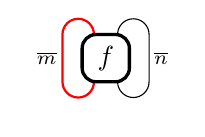
\begin{tikzpicture}[baseline=-.1cm, rotate=90]
	\draw[thick, red] (-.3,.15) arc (270:90:.2cm) -- (.3,.55) arc (90:-90:.2cm);
	\draw (-.3,-.15) arc (90:270:.2cm) -- (.3,-.55) arc (-90:90:.2cm);
	\roundNbox{unshaded}{(0,0)}{.3}{0}{0}{$f$}
%	\node at (-.7,-.35) {\scriptsize{$n$}};
	\node at (0,-.7) {\scriptsize{$\overline{n}$}};
	\node at (0,.75) {\scriptsize{$\overline{m}$}};
%	\node at (.7,.35) {\scriptsize{$m$}};
\end{tikzpicture}
\right)
\end{equation}
Where $n$ and $\overline{n}$ represent $\xalt$ and $\xbaralt$, respectively. This makes each $A_n$ a finite dimensional von Neumann algebra.

\begin{rem}
The aforementioned trace can be identified with a complex scalar exactly when $m$ is simple. Indeed the fist two cups define a morphism in $Hom_{\cC}(1, \overline{m}\otimes m)\otimes Hom_{\cC}( 1,  n \otimes \overline{n})$ but $\Hom_{\cC}(1,\overline{m}\otimes m)\cong \Hom_{\cC}(m,m)\cong \C$. Thus $\Hom_{\cC}(1,\overline{m}\otimes m)$ is one dimensional so there is some $i$ such that $\Hom_{\cC}(1,\overline{m}\otimes m)\cong \Hom_{\cC}(1_i,\overline{m}\otimes m)$. So the first two cups define a map whose source is isomorphic to $1_i$, and similarly the target is isomorphic to $1_i$, so it defines a map in $\End_{\cC}(1_i)$.
\end{rem}

We also have a natural inclusion $A_n \rightarrow A_{n+1}$ such that the trace restricts ($tr_{n+1}|_{A_n}=tr_n$):
\begin{equation}\label{eq:Inclusion}
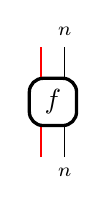
\begin{tikzpicture}[baseline=-.1cm, rotate=90]
	\draw[thick, red] (-.7,.15) -- (.7,.15);
	\draw (-.7,-.15) -- (.7,-.15);
	\roundNbox{unshaded}{(0,0)}{.3}{0}{0}{$f$}
	\node at (-.9,-.15) {\scriptsize{$n$}};
	\node at (.9,-.15) {\scriptsize{$n$}};
\end{tikzpicture}
\mapsto
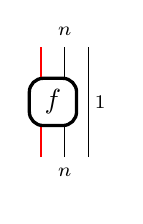
\begin{tikzpicture}[baseline=-.2cm, rotate=90]
	\draw[thick, red] (-.7,.15) -- (.7,.15);
	\draw (-.7,-.15) -- (.7,-.15);
	\draw (-.7,-.45) -- (.7,-.45);
	\roundNbox{unshaded}{(0,0)}{.3}{0}{0}{$f$}
	\node at (-.9,-.15) {\scriptsize{$n$}};
	\node at (.9,-.15) {\scriptsize{$n$}};
	\node at (0,-.6) {\scriptsize{$1$}};
\end{tikzpicture}
\end{equation}

The 1 indicates 1 string to the right (with appropriate shading). We also have a trace preserving conditional expectation $E_n:A_n\rightarrow A_{n-1}$ which acts a left inverse to the previously defined inclusion:

\begin{equation}\label{eq:ConditionalExpectationAn}
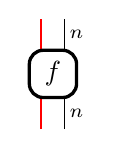
\begin{tikzpicture}[baseline=-.1cm]
	\draw[thick, red] (-.15,-.7) -- (-.15,.7);
	\draw (.15,-.7) -- (.15,.7);
	\roundNbox{unshaded}{(0,0)}{.3}{0}{0}{$f$}
	\node at (.3,.5) {\scriptsize{$n$}};
	\node at (.3,-.5) {\scriptsize{$n$}};
\end{tikzpicture}
\mapsto\,
\frac{1}{d}
\cdot
\left(\,\,
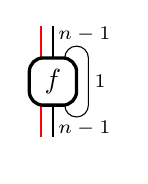
\begin{tikzpicture}[baseline=-.1cm]
	\draw[thick, red] (-.15,-.7) -- (-.15,.7);
	\draw (0,-.7) -- (0,.7);
	\draw (.15,.3) arc (180:0:.15cm) -- (.45,-.3) arc (0:-180:.15cm);
	\roundNbox{unshaded}{(0,0)}{.3}{0}{0}{$f$}
	\node at (.4,.6) {\scriptsize{$n-1$}};
	\node at (.4,-.6) {\scriptsize{$n-1$}};
	\node at (.6,0) {\scriptsize{$1$}};
\end{tikzpicture}
\right)
\end{equation}

Where $d:=\dim_{\cC}(x)=\dim_{\cC}(\overline{x})$, which is also the value of a closed loop appearing in the diagram. Given the previously defined inclusion and that multiplication is given by vertical stacking of diagrams it's clear that $E_n$ is $A_{n-1}$ bilinear. Similarly we have that $tr_n=tr_{n-1} \circ E_n$.

Finally we will define the jones projections for each inclusion $A_{n}\subset A_{n+1}$ is given by

\begin{equation}\label{eq:JonesProjections}
e_n=
\frac1d\cdot
\left(\,\,
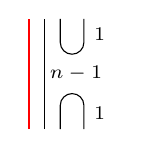
\begin{tikzpicture}[baseline=-.1cm]
	\draw[thick, red] (-.3,-.7) -- (-.3,.7);
	\draw (-.1,-.7) -- (-.1,.7);
	\draw (.1,-.7) -- (.1,-.4) arc (180:0:.15cm) -- (.4,-.7);
	\draw (.1,.7) -- (.1,.4) arc (-180:0:.15cm) -- (.4,.7);
%	\node at (-.1,-1) {\scriptsize{$n-1$}};
	\node at (.3,0) {\scriptsize{$n-1$}};
	\node at (.6,.5) {\scriptsize{$1$}};
	\node at (.6,-.5) {\scriptsize{$1$}};
\end{tikzpicture}
\right)
\in
A_{n+1}.
\end{equation}

Where the $n-1$ indicates $n-1$ vertical strands with appropriate shading to the right of the red strand. The Temperley-Lieb-
Jones relations follow immediately from the definition and the fact that closed loops count for a factor of $d$. Similarly 
for any $x\in A_n$ we have that: $e_nxe_n=E_n(x)e_n$. Clearly $E_{n+1}(e_n)=d^{-2}id_{m \otimes \xalt}$. Finally the pull 
down condition holds as for each $x\in A_{n+1}$ we have that $d^2 E_{n+1}(xe_n)e_n=xe_n$. Equivalently $A_{n} e_n A_n$ is a 
two sided ideal in $A_{n+1}$. Thus the tower algebras given by the $A_n$ is indeed a Markov sequence.
 
\begin{prop}
The Markov sequence of von Neumann Algebras $(A_n, tr_n)_{n\geq 0}$ is finite depth.
\end{prop}

\begin{proof}
$m\otimes \xalt$ generates $\cM$. Let $s^i_1,\ldots s^i_{r_i}$, for $i=0$ or $1$ be a collection of nonisomorphic simple objects in $\cC_{2i}$ such that every object in $\cC_{2i}$ is isomorphic to a direct sum of these elements. 

Recall that $\Hom_{\cC}(s^i_k,s^i_l)\cong \delta_{kl}\bbC$, thus:

$$\End_{\cC}(m\otimes\xalt)\cong \bigoplus\limits_{j}\End_{\cC}(n_j s^i_j) \cong \bigoplus\limits_{j}M_{n_j}(\bbC)$$
If we have that 
$$m \otimes \xalt \cong \bigoplus\limits_{j}n_js^i_j$$
where $i$ is 0 if $n$ is even and odd if $n$ is 1, and where:
$$n_js^i_j:=\underbrace{s^i_j\oplus s^i_j\oplus \cdots \oplus s^i_j}_{n_j \,\, \text{summands}}$$

Thus at each level of the Bratelli diagram corresponding to $A_n$ there are at most $\max\{r_1,r_0\}$ vertices, so the principal graph must be finite.
\end{proof}

\begin{thm}
The principal graph obtained from the Markov sequence $(A_n)_{n\geq 0}$ is independent of the choice of $m$.
\end{thm}

\section{The Embedding Theorem}

\begin{claim*}
A subfactor planar algebra can be embedded into the bipartite graph planar algebra of the principle graph obtained by right-acting the subfactor planar algebra on a cyclic module.
\end{claim*}
From the paper of Penneys and Jones we see that for any strongly markov tower of algebras, we can construct a canonical relative commutant planar algebra. It was shown that this planar algebra was isomorphic to the bipartite graph planar algebra of the Bratelli diagram of the first inclusion in the tower. We have shown that the inclusions of $\left(A_{n}\right)$ are eventually standard (the tower $\left(A_{n}\right)$ is of finite depth). Thus if we fix a number $s=2r$ such that the inclusion $A_{2r} \subset A_{2r+1} \subset A_{2r+2}$ is standard, then the canonical relative commutant planar algebra constructed on the strongly markov tower $B_{n}=A_{2r+n}$ would be isomorphic to the bipartite graph planar algebra of the principle graph of the tower $\left(A_{n}\right)$ (The principle graph of $A_{n}$ is the Bratelli diagram of the first inclusion in $\left(B_{n}\right)$).\\

If we denote the canonical relative commutant planar algebra on $\left(B_{n}\right)$ by $P_{\bullet}$, then by construction we have the following:
\begin{align*}
	P_{n,+} &=  A'_{2r}\cap A_{2r+n} \\
	P_{n,-}  &= A'_{2r+1}\cap A_{2r+n+1} 
\end{align*}

Consider the linear extension of following map, $\Phi$, which puts $2r$ strings on the left of elements of $Q_{n,+}$  and $2r+1$ strings on the left of elements of $Q_{n,-}$\todo{insert picture here} \\ 

This map sends $Q_{n , +}$ to $P_{n,+}$ and $Q_{n , -}$ to $P_{n,-}$. In order to check that $\Phi$ is a planar embedding map, we use Lemma 2.48 in the paper of Penneys and Jones. We denote traces in $Q_{\bullet}$ by $\overline{\tr}$ and traces in $P_{\bullet}$ by $\tr$. We denote the Jones projections in $Q_{\bullet}$ by $E_{j}$ and the Jones projections in  $P_{\bullet}$ by $F_{j}$.

\begin{thm}
The image of the map $\Phi:Q_{\bullet} \to P_{\bullet}$ is a sub $\dagger$-planar algebra of $P_{\bullet}$.
\end{thm} 

\begin{proof}
Observe that for all $x,y \in Q_{\bullet}$, we have that 
\begin{align*}
	\Phi(x^{*}) &= \Phi(x)^{\dagger} \\
	\Phi(xy) &= \Phi(x)\Phi(y) \\
	\overline{\tr}_{n}(x) &= \frac{1}{\dim_\cC(x)^{2r}}\cdot\tr_{n}(\Phi(x)) 
\end{align*}
To prove injectivity we can use the faithfullness of the traces and the third equation displayed above. \\
\begin{enumerate}[(1)]
\item By the construction of $P_{\bullet}$ we have that $\Phi(E_j)=F_j$. Thus $\Phi(Q_{\bullet})$ is closed under multiplication by Jones projections. \\ 
\item \begin{enumerate}[(i)]
\item We have that $\Phi(E_n(x)) = E_2r+n(\Phi(x))$. This follows from the graphical calculi in both the domain and range. Thus $\Phi(Q_{\bullet})$ is closed under conditional expectation. We also have that $E_{2r+n | Q'_{2r}\cap Q_{2r+n}} = E_{P_{n,+}}$ because they both are faithful trace preserving conditional expectations on $P_{n,+}$\\ 
\item We have that $\Phi(\beta_n(x)) = \beta_2r+n(\Phi(x))$ due to graphical calculi in the domain and range. Also note that the inclusion from $P_{n,+} \to P_{n+1,+}$ is just the restriction of the incusion from $Q_{2r+n,+} \to Q_{2r+n+1,+}$. \\ 
\item \todo{left capping via pimsner popa bases} \\
\end{enumerate}
\item The negative inclusion $i^{-}_{n} : P_{n,-} \to P_{n+1,+}$ is just the identity on the relative commutant planar algebra. Graphically this is equivalent to adding a string on the left. Let $\overline{i^{-}_{n}}$ be the negative inclusion in $Q_{\bullet}$. Thus we have that for x in $Q_{n,-}$.
\[ i^{-}_{n}(\Phi(x)) = \Phi(x) = \Phi(\overline{i^{-}_{n}}(x)) \]
\end{enumerate}
\end{proof}

We have checked that $\Phi(Q_{\bullet}) \subset P_{\bullet}$ is a $\dagger$-planar algebra inclusion. Let $G_\bullet$ be the bipartite graph planar algebra on the principle graph of $(A_n)$. Then by Theorem 3.33 in the paper of Penneys and Jones, we have that $P_\bullet$ is $\dagger$-planar algebra isomorphic to $G_\bullet$. Thus we have succesfully embedded $Q_\bullet$ into $G_\bullet$.

\begin{cor}[The Embedding Theorem]
A subfactor planar algebra can be embedded into the bipartite graph planar algebra of the principle graph obtained by right-acting the subfactor planar algebra on a cyclic module.
\end{cor}

\end{document}
